
% packages
\documentclass[12pt, letterpaper]{article}
\usepackage[utf8]{inputenc}
\usepackage[T1]{fontenc}
\usepackage[document]{ragged2e}
\usepackage{amsmath}
\usepackage{fullpage}
\usepackage{color}
\usepackage[table]{xcolor}
\usepackage{listings}
\usepackage{graphicx}

\lstset{
  aboveskip=3mm,
  belowskip=-2mm,
  backgroundcolor=\color{white},
  basicstyle=\footnotesize,
  breakatwhitespace=false,
  breaklines=true,
  captionpos=b,
  commentstyle=\color{red},
  deletekeywords={...},
  escapeinside={\%*}{*)},
  extendedchars=true,
  framexleftmargin=16pt,
  framextopmargin=3pt,
  framexbottommargin=6pt,
  frame=tb,
  keepspaces=true,
  keywordstyle=\color{blue},
  language=scilab,
  literate=
  {á}{{\'a}}1 {é}{{\'e}}1 {í}{{\'i}}1 {ó}{{\'o}}1 {ú}{{\'u}}1
  {Á}{{\'A}}1 {É}{{\'E}}1 {Í}{{\'I}}1 {Ó}{{\'O}}1 {Ú}{{\'U}}1
  {à}{{\`a}}1 {è}{{\`e}}1 {ì}{{\`i}}1 {ò}{{\`o}}1 {ù}{{\`u}}1
  {À}{{\`A}}1 {È}{{\'E}}1 {Ì}{{\`I}}1 {Ò}{{\`O}}1 {Ù}{{\`U}}1
  {ä}{{\"a}}1 {ë}{{\"e}}1 {ï}{{\"i}}1 {ö}{{\"o}}1 {ü}{{\"u}}1
  {Ä}{{\"A}}1 {Ë}{{\"E}}1 {Ï}{{\"I}}1 {Ö}{{\"O}}1 {Ü}{{\"U}}1
  {â}{{\^a}}1 {ê}{{\^e}}1 {î}{{\^i}}1 {ô}{{\^o}}1 {û}{{\^u}}1
  {Â}{{\^A}}1 {Ê}{{\^E}}1 {Î}{{\^I}}1 {Ô}{{\^O}}1 {Û}{{\^U}}1
  {œ}{{\oe}}1 {Œ}{{\OE}}1 {æ}{{\ae}}1 {Æ}{{\AE}}1 {ß}{{\ss}}1
  {ű}{{\H{u}}}1 {Ű}{{\H{U}}}1 {ő}{{\H{o}}}1 {Ő}{{\H{O}}}1
  {ç}{{\c c}}1 {Ç}{{\c C}}1 {ø}{{\o}}1 {å}{{\r a}}1 {Å}{{\r A}}1
  {€}{{\EUR}}1 {£}{{\pounds}}1,
  morekeywords={*,...},
  numbers=left,
  numbersep=10pt,
  numberstyle=\tiny\color{black},
  rulecolor=\color{black},
  showspaces=false,
  showstringspaces=false,
  showtabs=false,
  stepnumber=1,
  stringstyle=\color{gray},
  tabsize=4,
  title=\lstname,
}

% Document information
\title{Mini Projet}
\author{Nicolas BOUTON}

% Begin document
\begin{document}

\maketitle

\begin{enumerate}

  % Question 1
\item Nous avons le système suivant :

  \begin{equation*}
    \left\{
    \begin{array}{l}
      u'(t) = - u(t) \\
      u(0) = 1
    \end{array}
    \right.
  \end{equation*}

  \begin{equation*}
    \begin{array}{l}
      u(t) = ke^{-t} \\
      u(t = 0) = 1 = k e^0 = k \\
      u(t) = e^{-t}
    \end{array}
  \end{equation*}

  % Question 2
\item Appliquons la méthode d'Euler explicite :

  \begin{equation*}
    \begin{split}
      u_{m + 1} & = u_m + \Delta t f(u_m) \\
      & = u_m + \Delta t (- u_m) \\
      & = u_m ( 1 - \Delta t ) \\
    \end{split}
  \end{equation*}

  Nous remarquons que c'est une suite géométique de raison $ 1 -
  \Delta t$. Donc on en déduit que $\forall m \in [0, n], u_m = ( 1 -
  \Delta t )^m$


  % Question 3
\item
  Calculons la solution exacte en $t = 1$ :

  \begin{equation*}
    u(1) = e^{-1} \approx 0,37
  \end{equation*}

  Maintenant essayons de voir la convergence de la solution trouvé
  avec la méthode d'Euler explicite :

  On pose $\Delta t = \frac{1}{n}$

  \begin{equation*}
    \begin{split}
      u_n & = ( 1 - \Delta t )^n \\
      & = \left( 1 - \frac{1}{n} \right)^n
    \end{split}
  \end{equation*}

  \begin{equation*}
    \lim_{\Delta t \rightarrow 0} {u_n}
    =
    \lim_{n \rightarrow +\infty} {u_n}
    =
    \lim_{n \rightarrow +\infty} {\left( 1 - \frac{1}{n} \right)^n}
    =
    \lim_{n \rightarrow +\infty} {1^n}
    =
    0
  \end{equation*}

  Donc on en conclu que lorsque $\Delta t$ tend vers 0, alors $u_m$
  converge vers 0.

  % Question 4
\item

  Appliquons le développenment limité de taylor :

  \begin{equation*}
    \begin{split}
      u(t_m) & = u(t_{m + 1}) + u'(t_{m+1}) (t_m - t_{m+1}) + O(t_m -
      t_{m+1}) \\
      & = u(t_{m + 1}) + u'(t_{m+1}) (- \Delta t) + O(- \delta t) \\
      & = u(t_{m + 1}) - u'(t_{m+1}) \Delta t \\
      u'(t_{m+1}) & = \frac{u(t_{m + 1}) - u(t_m)}{\Delta t}
    \end{split}
  \end{equation*}

  Et on a $u'(t_{m+1}) = f(u(t_{m+1})) = - u(t_{m+1})$

  Donc

  \begin{equation*}
    \frac{u(t_{m + 1}) - u(t_m)}{\Delta t} = u'(t_{m+1}) \approx
    f(u(t_{m+1}))
  \end{equation*}


  % Question 5
\item
  Le schéma d'euler implicite :

  \begin{equation*}
    u(t_{m+1}) = u(t_m) + \Delta t f(u(t_{m+1}))
  \end{equation*}


  % Question 6
\item

  D'après la question précédentes on a :

  \begin{equation*}
    \begin{split}
      u(t_{m+1}) & = u(t_m) + \Delta t f(u(t_{m+1})) \\
      u(t_m) & = u(t_{m+1}) - \Delta t f(u(t_{m+1})) \\
      u(t_m) & = u(t_{m+1}) + \Delta t u(t_{m+1}) \\
      u(t_m) & = u(t_{m+1}) (1 + \Delta t) \\
      u(t_{m+1}) & = \frac{u(t_m)}{(1 + \Delta t)} \\
      u(t_m) & = \frac{u(t_{m-1})}{(1 + \Delta t)} \\
      u(t_m) & = \frac{1}{(1 + \Delta t)^m} \\
    \end{split}
  \end{equation*}


  % Question 7
\item
  Partons d'Euler explicite :

  \begin{equation*}
    \begin{split}
      u_{m+1} & = u_m + \Delta t f(u_m) \\
      \frac{u_{m+1} - u_m}{\Delta t} = f(u_m)
    \end{split}
  \end{equation*}

  or on a :

  \begin{equation*}
    \frac{u(t_{m + 1}) - u(t_m)}{\Delta t} = f(u(t_{m+1}))
  \end{equation*}

  Donc

  \begin{equation*}
    \frac{u(t_{m + 1}) - u(t_m)}{\Delta t} = \frac{f(u(t_{m+1})) + f(u(t_m))}{2}
  \end{equation*}

    
  % Question 8
\item

  D'après la question précédentes on a :

  \begin{equation*}
    \begin{split}
      \frac{u(t_{m + 1}) - u(t_m)}{\Delta t} & = \frac{f(u(t_{m+1})) +
        f(u(t_m))}{2} \\
      u(t_{m + 1}) - u(t_m) & = \frac{\Delta t f(u(t_{m+1})) +
        \Delta t f(u(t_m))}{2} \\
      u(t_{m + 1}) - \frac{1}{2} \Delta t f(u(t_{m+1})) & = u(t_m) +
      \frac{1}{2} \Delta t f(u(t_m)) \\
    \end{split}
  \end{equation*}

  % Question 9
\item

  D'après la question précédentes on a :

  \begin{equation*}
    \begin{split}
        u(t_{m + 1}) - \frac{1}{2} \Delta t f(u(t_{m+1})) & = u(t_m) +
        \frac{1}{2} \Delta t f(u(t_m)) \\
        u(t_{m + 1}) + \frac{1}{2} \Delta t u(t_{m+1}) & = u(t_m) -
        \frac{1}{2} \Delta t u(t_m) \\
        u(t_{m + 1}) \left(1 + \frac{1}{2} \Delta t \right) & = u(t_m) \left( 1 -
        \frac{1}{2} \Delta t \right) \\
        u(t_{m + 1})  & = u(t_m) \left( \frac{1 - \frac{1}{2} \Delta
          t}{1 + \frac{1}{2} \Delta t} \right) \\
        u(t_{m + 1})  & = u(t_m) \left( \frac{1 - \frac{1}{2} \Delta
          t}{1 + \frac{1}{2} \Delta t} \right) \\
        u(t_{m + 1})  & = u(t_m) \left( \frac{\frac{2 - \Delta
          t}{2} }{\frac{2 + \Delta t}{2}} \right) \\
        u(t_{m + 1})  & = u(t_m) \left( \frac{2 - \Delta
          t}{2 + \Delta t} \right) \\
    \end{split}
  \end{equation*}

  Donc

  \begin{equation*}
    \begin{split}
      u_{m + 1}  & = u_m \left( \frac{2 - \Delta
        t}{2 + \Delta t} \right) \\
      u_m  & = u_{m-1} \left( \frac{2 - \Delta
        t}{2 + \Delta t} \right) \\
      u_m  & = \left( \frac{2 - \Delta
        t}{2 + \Delta t} \right)^m \\
    \end{split}
  \end{equation*}

  % Question 10
\item

  Calculons la solutionà $t = 1$:

  \begin{equation*}
    u(1) = e^{-1} \approx 0,37
  \end{equation*}

  Supposons que $\Delta t$ est petit, c'est-à-dire $\Delta t =
  \frac{1}{n}$ \newline

  \underline{Schéma d'Euler explicite :}

  \begin{equation*}
    u_n = \left( 1 - \frac{1}{n} \right)^n
  \end{equation*}

  \underline{Schéma d'Euler implicite :}

  \begin{equation*}
    u_n = \frac{1}{\left( 1 + \frac{1}{n} \right)^n}
  \end{equation*}

  \underline{Schéma numérique :}

  \begin{equation*}
    u_n = \left( \frac{2 - \frac{1}{n}}{2 + \frac{1}{n}} \right)^n
  \end{equation*}

  Ces schéma sont implémente dans \textbf{main.f90}.

  \newpage

  \lstinputlisting[language=fortran]{main.f90}

  En exécutant ce code on obtient :

  \lstinputlisting{result.txt}

  Ici on a choisis $n_1 = 10$ et $n_2 = 100$. On voit que pour les
  schémas d'Euler le delta est de l'ordre de $10^{-2}$ et que pour le
  schéma numérique il est de l'ordre de $10^{-4}$.\newline
  Donc on peut supposer que si les erreurs absolus des schémas
  d'Euler sont de l'ordre de $k \Delta t$ alors l'erreur absolue du
  schéma numérique est de l'ordre de $k \Delta t^2$.


  Le programme \textbf{etude\_1.sci} permet de générer les graphes
  suivants :

  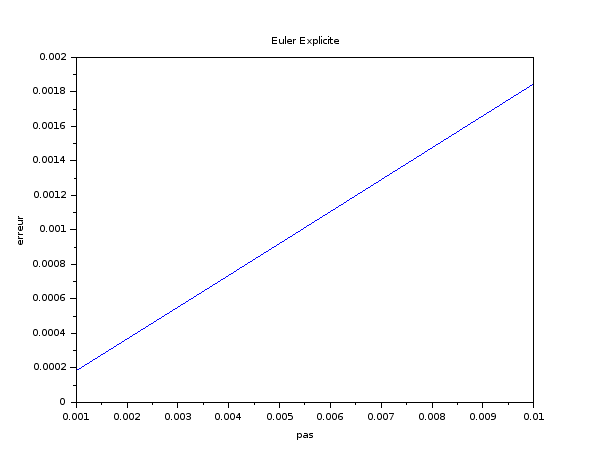
\includegraphics[scale = 0.6]{img/etude_1_ee.png}

  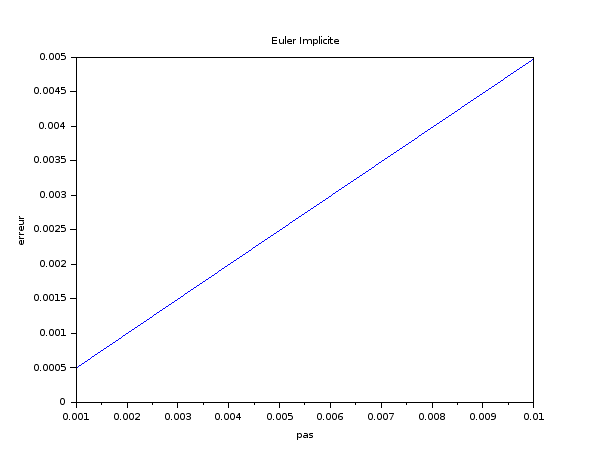
\includegraphics[scale = 0.6]{img/etude_1_ei.png}

  On peut voir que les erreurs relatives des schémas d'Euler suivent
  un ordre linéaire donc $k \Delta t$.

  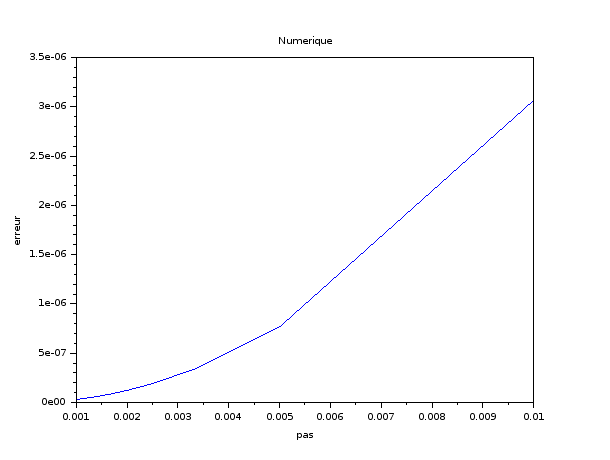
\includegraphics[scale = 0.6]{img/etude_1_num.png}

  On peut voir que l'erreur relative du schéma numérique suit un ordre
  quadratique donc $k \Delta t^2$.

  
  % Question 11
\item

  \underline{Solution exacte :}

  \begin{equation*}
    \left\{
    \begin{array}{l}
      u'(t) = - u^2 (t) \\
      u(0) = 1
    \end{array}
    \right.
  \end{equation*}

  On trouve :

  \begin{equation*}
    u(t) = - \frac{1}{- t + k}
  \end{equation*}

  Et on a :

  \begin{equation*}
    u(0) = 1 = - \frac{1}{k}
  \end{equation*}

  Donc 

  \begin{equation*}
    k = - 1
  \end{equation*}

  Et donc

  \begin{equation*}
    u(t) = \frac{1}{t + 1}
  \end{equation*}


  \underline{Euler explicite :}

  \begin{equation*}
    \begin{split}
      u_{m+1} & = u_m + \Delta t f(u_m) \\
      & = u_m + \Delta t ( - u_m^2) \\
      & = u_m - \Delta t u_m^2 \\
      & = u_m (1 - \Delta t u_m) \\
    \end{split}
  \end{equation*}

  Donc $u_m = u_{m-1} (1 - \Delta t u_{m-1})$

  \underline{Euler implicite :}

  \begin{equation*}
    \begin{split}
      u_{m+1} & = u_m + \Delta t f(u_{m+1}) \\
      & = u_m + \Delta t ( - u_{m+1}^2) \\
      & = u_m - \Delta t u_{m+1}^2 \\
      \Delta t u_{m+1}^2 + u_{m+1} - u_m & = 0\\
    \end{split}
  \end{equation*}

  Calculons le discriminant :

  \begin{equation*}
    \begin{split}
      \Delta & = b^2 - 4ac \\
      & = 1^2 - 4 \Delta t (- u_m) \\
      & = 4 \Delta t u_m + 1\\
    \end{split}
  \end{equation*}

  Le résustat de $u_{m+1}$ est la solution poisitive :

  \begin{equation*}
    \begin{split}
      u_{m+1} & = \frac{- b + \sqrt{\Delta}}{2a} \\
      & = \frac{- 1 + \sqrt{4 \Delta t u_m + 1}}{2 \Delta t} \\
      & = \frac{\sqrt{4 \Delta t u_m + 1} - 1}{2 \Delta t} \\
    \end{split}
  \end{equation*}

  Donc $ u_{m+1} = \frac{\sqrt{4 \Delta t u_m + 1} - 1}{2 \Delta t}$
  et $ u_m = \frac{\sqrt{4 \Delta t u_{m-1} + 1} - 1}{2 \Delta t}$
  
  Le programme \textbf{etude\_2.sci} permet de générer les graphes
  suivants :

  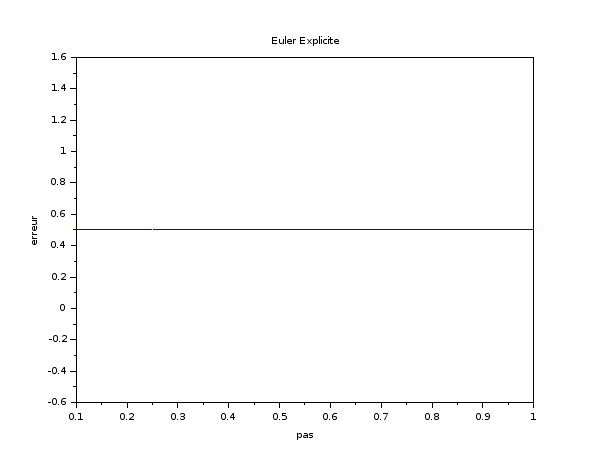
\includegraphics[scale = 0.6]{img/etude_2_ee.png}

  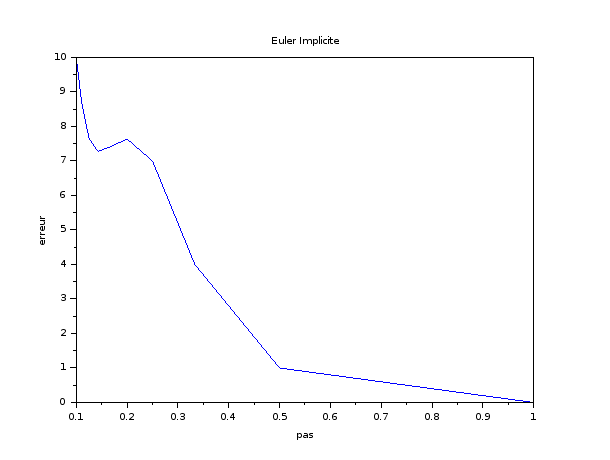
\includegraphics[scale = 0.6]{img/etude_2_ei.png}

  J'ai sûrement dû faire une erreur car pour \textbf{euler explicite}
  j'ai une droite constante horizontale, c'est-à-dire que toutes les
  erreurs sont égales. Mais je l'ai fait avec des petites tailles car
  sinon \textbf{scilab} crashais car la récursion faisait appelle a
  trop de fonction.

  % Question 12
\item
  Cette question est lié à la précédente donc de ce que je vois, si
  c'est bon, nous avons pas les mêmes conclusions que dans le cas
  linéaire initiale.
  
\end{enumerate}

\end{document}
